\section{Modello di sviluppo}
La scelta del modello di sviluppo\glosp è una delle realtà fondamentali per la realizzazione di un progetto software.
Avendo una visione abbastanza chiara dell'intero progetto e, allo stesso tempo, una limitata conoscenza dei requisiti specifici, si è scelto di seguire il \textbf{modello incrementale}.

\subsection{Modello incrementale}

\begin{figure}[H]
	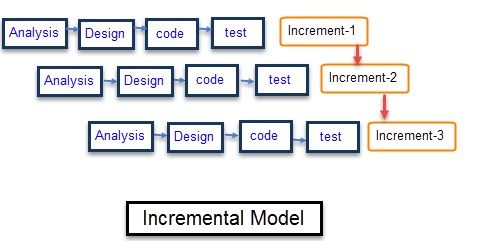
\includegraphics[width=0.99\linewidth]{res/images/incremental_model.jpg}
	\caption{Modello di sviluppo incrementale - \url{https://www.guru99.com/}}
\end{figure}

Il modello di sviluppo incrementale permette la suddivisione del progetto in più sottoinsiemi,
ognuno dei quali incorpora una funzionalità diversa che, se necessario, verrà migliorata ad ogni incremento.  \\
Ad ogni incremento del sistema è consentita la modifica, aggiunta ed eliminazione di requisiti in base alle esigenze progettuali; 
è necessario un colloquio diretto con il proponente per approvare tali cambiamenti. \\
Utilizzando questo modello di sviluppo il versionamento del sistema è reso semplice e intuitivo, in quanto ogni modifica è facilmente tracciabile da un incremento all'altro e se ne possono valutare direttamente i difetti o benefici.\\
I vantaggi predisposti dal modello incrementale sono i seguenti:
\begin{itemize}
	\item gli incrementi sono disposti in base alle funzionalità con priorità decrescente, partendo da quelle con priorità e impatto maggiori
	così da avere subito un riscontro diretto;
	\item ogni incremento genera un risultato che può essere valutato dal proponente, approvandone i benefici o evidenziandone i difetti;
	\item rende sempre disponibile una recente baseline\glosp per una eventuale rivalutazione, senza dover ripercorrere tutti i passi effettuati fino ad ora dall'inizio dello sviluppo;
	\item tutti gli errori sono limitati al singolo incremento;
	\item le modifiche e le correzioni sono molto economiche in quanto di facile reperibilità;
	\item le fasi di test sono mirate al corrente incremento, quindi più efficienti.
\end{itemize}
Sono presenti anche degli aspetti negativi per quanto riguarda il modello incrementale. La suddivisione di un singolo problema in più parti, dove almeno una di esse richiede una modifica, comporta una nuova elaborazione anche delle altre parti che non sono direttamente coinvolte, ciò aumenta in modo considerevole i tempi di sviluppo.
I problemi potrebbero derivare anche dall'architettura del sistema, la quale potrebbe non riuscire a soddisfare tutti i requisiti raccolti in anticipo per l'intero ciclo di vita del software.

\subsection{Incrementi individuati}
Durante i periodi di Progettazione e Codifica per la Technology Baseline\glosp e Progettazione di Dettaglio sono stati individuati alcuni incrementi. Di seguito è riportato il tracciamento incremento-requisiti, in maniera tale da comprendere meglio quali requisiti vengono soddisfatti in ciascun incremento. I requisiti riportati nella tabella includono tutti i requisiti figli. Tutti i requisiti non riportati nella tabella sono da intendersi soddisfatti, in parte, da ogni incremento. Tali requisiti sono reperibili all’interno del documento \textit{Analisi dei Requisiti v4.0.0}.


\counterwithin{table}{section}
\renewcommand{\arraystretch}{1.5}
\rowcolors{2}{dispari}{pari}
\arrayrulecolor{white}
\begin{longtable}{ 
		>{\centering}p{0.17\textwidth} 
		>{\raggedright}p{0.28\textwidth}
		>{\raggedright}p{0.29\textwidth} 
		>{\centering}p{0.15\textwidth}
	}
	
	
	\caption{Tabella del tracciamento incremento-requisiti}\\
	\rowcolorhead
	\colorhead\textbf{Incremento} & \centering\colorhead\textbf{Requisiti}
	\tabularnewline
	\endfirsthead
	\rowcolor{white}\caption[]{(continua)}\\
	\rowcolorhead
	\colorhead\textbf{Incremento} & \centering\colorhead\textbf{Requisiti}
	\tabularnewline
	\endhead
	
	%R---------------------------------------------------------
	{Registrazione} & \centering RFO2\\
	\tabularnewline
	%R---------------------------------------------------------
	{Login} & \centering RFO3\\
	\tabularnewline
	%R---------------------------------------------------------
	{Logout} & \centering RFO4\\
	\tabularnewline
	%R---------------------------------------------------------
	{Home} & \centering RFO5\\
	\tabularnewline
	%R---------------------------------------------------------
	{Profilo utente} & \centering RFO7\\
	\tabularnewline
	%R---------------------------------------------------------
	{Progress Bar} & \centering RFF8\\
	\tabularnewline

\end{longtable}
\counterwithin{table}{subsection}	
\renewcommand{\arraystretch}{1}
\pagebreak

I requisiti sopracitati sono stati successivamente assegnati al relativo incremento. Quest'operazione è stata ritenuta utile al fine di organizzare meglio il lavoro. Viene riportata di seguito la tabella del tracciamento incremento-casi d'uso, in cui i casi d'uso riportati includono tutti i casi d’uso figli.

\counterwithin{table}{section}
\renewcommand{\arraystretch}{1.5}
\rowcolors{2}{dispari}{pari}
\arrayrulecolor{white}
\begin{longtable}{ 
		>{\centering}p{0.17\textwidth} 
		>{\raggedright}p{0.28\textwidth}
		>{\raggedright}p{0.29\textwidth} 
		>{\centering}p{0.15\textwidth}
	}
	
	
	\caption{Tabella del tracciamento incremento-casi d'uso}\\
	\rowcolorhead
	\colorhead\textbf{Incremento} & \centering\colorhead\textbf{Casi d'uso}
	\tabularnewline
	\endfirsthead
	\rowcolor{white}\caption[]{(Casi d'uso)}\\
	\rowcolorhead
	\colorhead\textbf{Incremento} & \centering\colorhead\textbf{Casi d'uso}
	\tabularnewline
	\endhead
	
	%R---------------------------------------------------------
	{Registrazione} & \centering UC1\\
	\tabularnewline
	%R---------------------------------------------------------
	{Login} & \centering UC6\\
	\tabularnewline
	%R---------------------------------------------------------
	{Logout} & \centering UC9\\
	\tabularnewline
	%R---------------------------------------------------------
	{Home} & \centering UC10\\
	\tabularnewline
	%R---------------------------------------------------------
	{Profilo utente} & \centering UC15\\
	\tabularnewline
	%R---------------------------------------------------------
	{Progress Bar} & \centering UC17\\
	\tabularnewline
	
\end{longtable}
\counterwithin{table}{subsection}	
\renewcommand{\arraystretch}{1}

Altri incrementi riguardanti la Gamification\glosp sono riportati nella relativa sezione del periodo in cui sono effettuati.
